\chapter{Model Optimization and Productionization}

\section{Optimization for the Edge}
Industrial monitoring often requires deployment on edge gateways (e.g., Raspberry Pi or NVIDIA Jetson) where resources are limited. We optimized our pipeline for these environments.

\subsection{Feature Dimensionality Reduction}
As discussed in Section 4, reducing the feature set from 104 to 40 decreased the memory footprint and CPU utilization by over 50\% with minimal accuracy loss. This allows the feature extraction script to run in near real-time on low-power devices.

\subsection{XGBoost vs. Deep Learning Trade-offs}
For production, the choice of model depends on the hardware budget:
\begin{table}[H]
    \centering
    \caption{Production Trade-offs}
    \begin{tabular}{@{}lccc@{}}
        \toprule
        \textbf{Metric} & \textbf{XGBoost (Edge)} & \textbf{SSLAM (Mid)} & \textbf{EfficientNet (Cloud)} \\ \midrule
        Macro F1-Score & 0.9234 & 0.9412 & 0.9937 \\
        Inference Latency & <1 ms & ~5 ms (GPU) & ~25 ms (GPU) \\
        Model Size & 2.4 MB & 12 MB & 45 MB \\
        Ideal Platform & Industrial Gateway & Jetson Nano & Central Server \\ \bottomrule
    \end{tabular}
\end{table}

\section{Inference Pipeline Design}
We developed a complete inference service using FastAPI to wrap our serialized models. 

\subsection{Service Workflow}
The inference service operates through a simple POST endpoint:
\begin{enumerate}
    \item \textbf{Receive:} Accepts a \texttt{.wav} file payload.
    \item \textbf{Preprocess:} Normalizes and standardizes the audio.
    \item \textbf{Extract:} Computes the Top 40 acoustic manifold features.
    \item \textbf{Predict:} Passes features to the XGBoost model or spectrogram to the EfficientNet model.
    \item \textbf{Response:} Returns the class label (e.g., "Machine 2 Abnormal") and a confidence score.
\end{enumerate}

\section{High-Performance Cloud Scaling with Modal}
While the XGBoost model is optimized for edge gateways, the high-capacity ResNet-34 and EfficientNet models are deployed using the \textbf{Modal} serverless GPU platform. This cloud-native architecture allows for:
\begin{itemize}
    \item \textbf{On-Demand Scaling:} GPU resources (NVIDIA A10G) are provisioned instantly upon request, ensuring low latency during bursts of diagnostic demand.
    \item \textbf{Diagnostic Visualization:} The API returns not only the classification result but also raw \textbf{waveform segments} and \textbf{internal feature maps} (from the ResNet Diagnostic Mode). This data is used to populate a centralized monitoring dashboard for engineers.
    \item \textbf{Persistence:} Model checkpoints and logs are stored in Modal Volumes, facilitating continuous integration and model versioning.
\end{itemize}

\section{Reliability and Monitoring}
The production service includes logging and performance monitoring. By tracking the distribution of confidence scores, we can detect "Concept Drift"—where the machine's acoustic signature slowly changes over years due to natural aging—and trigger a retraining cycle.

\subsection{Automated Performance Diagnostics}
To ensure the reliability of every training run and model update, our pipeline includes automated diagnostic generation. For every training iteration, a high-resolution confusion matrix is generated and exported to the \texttt{outputs/} directory.

\begin{figure}[H]
    \centering
    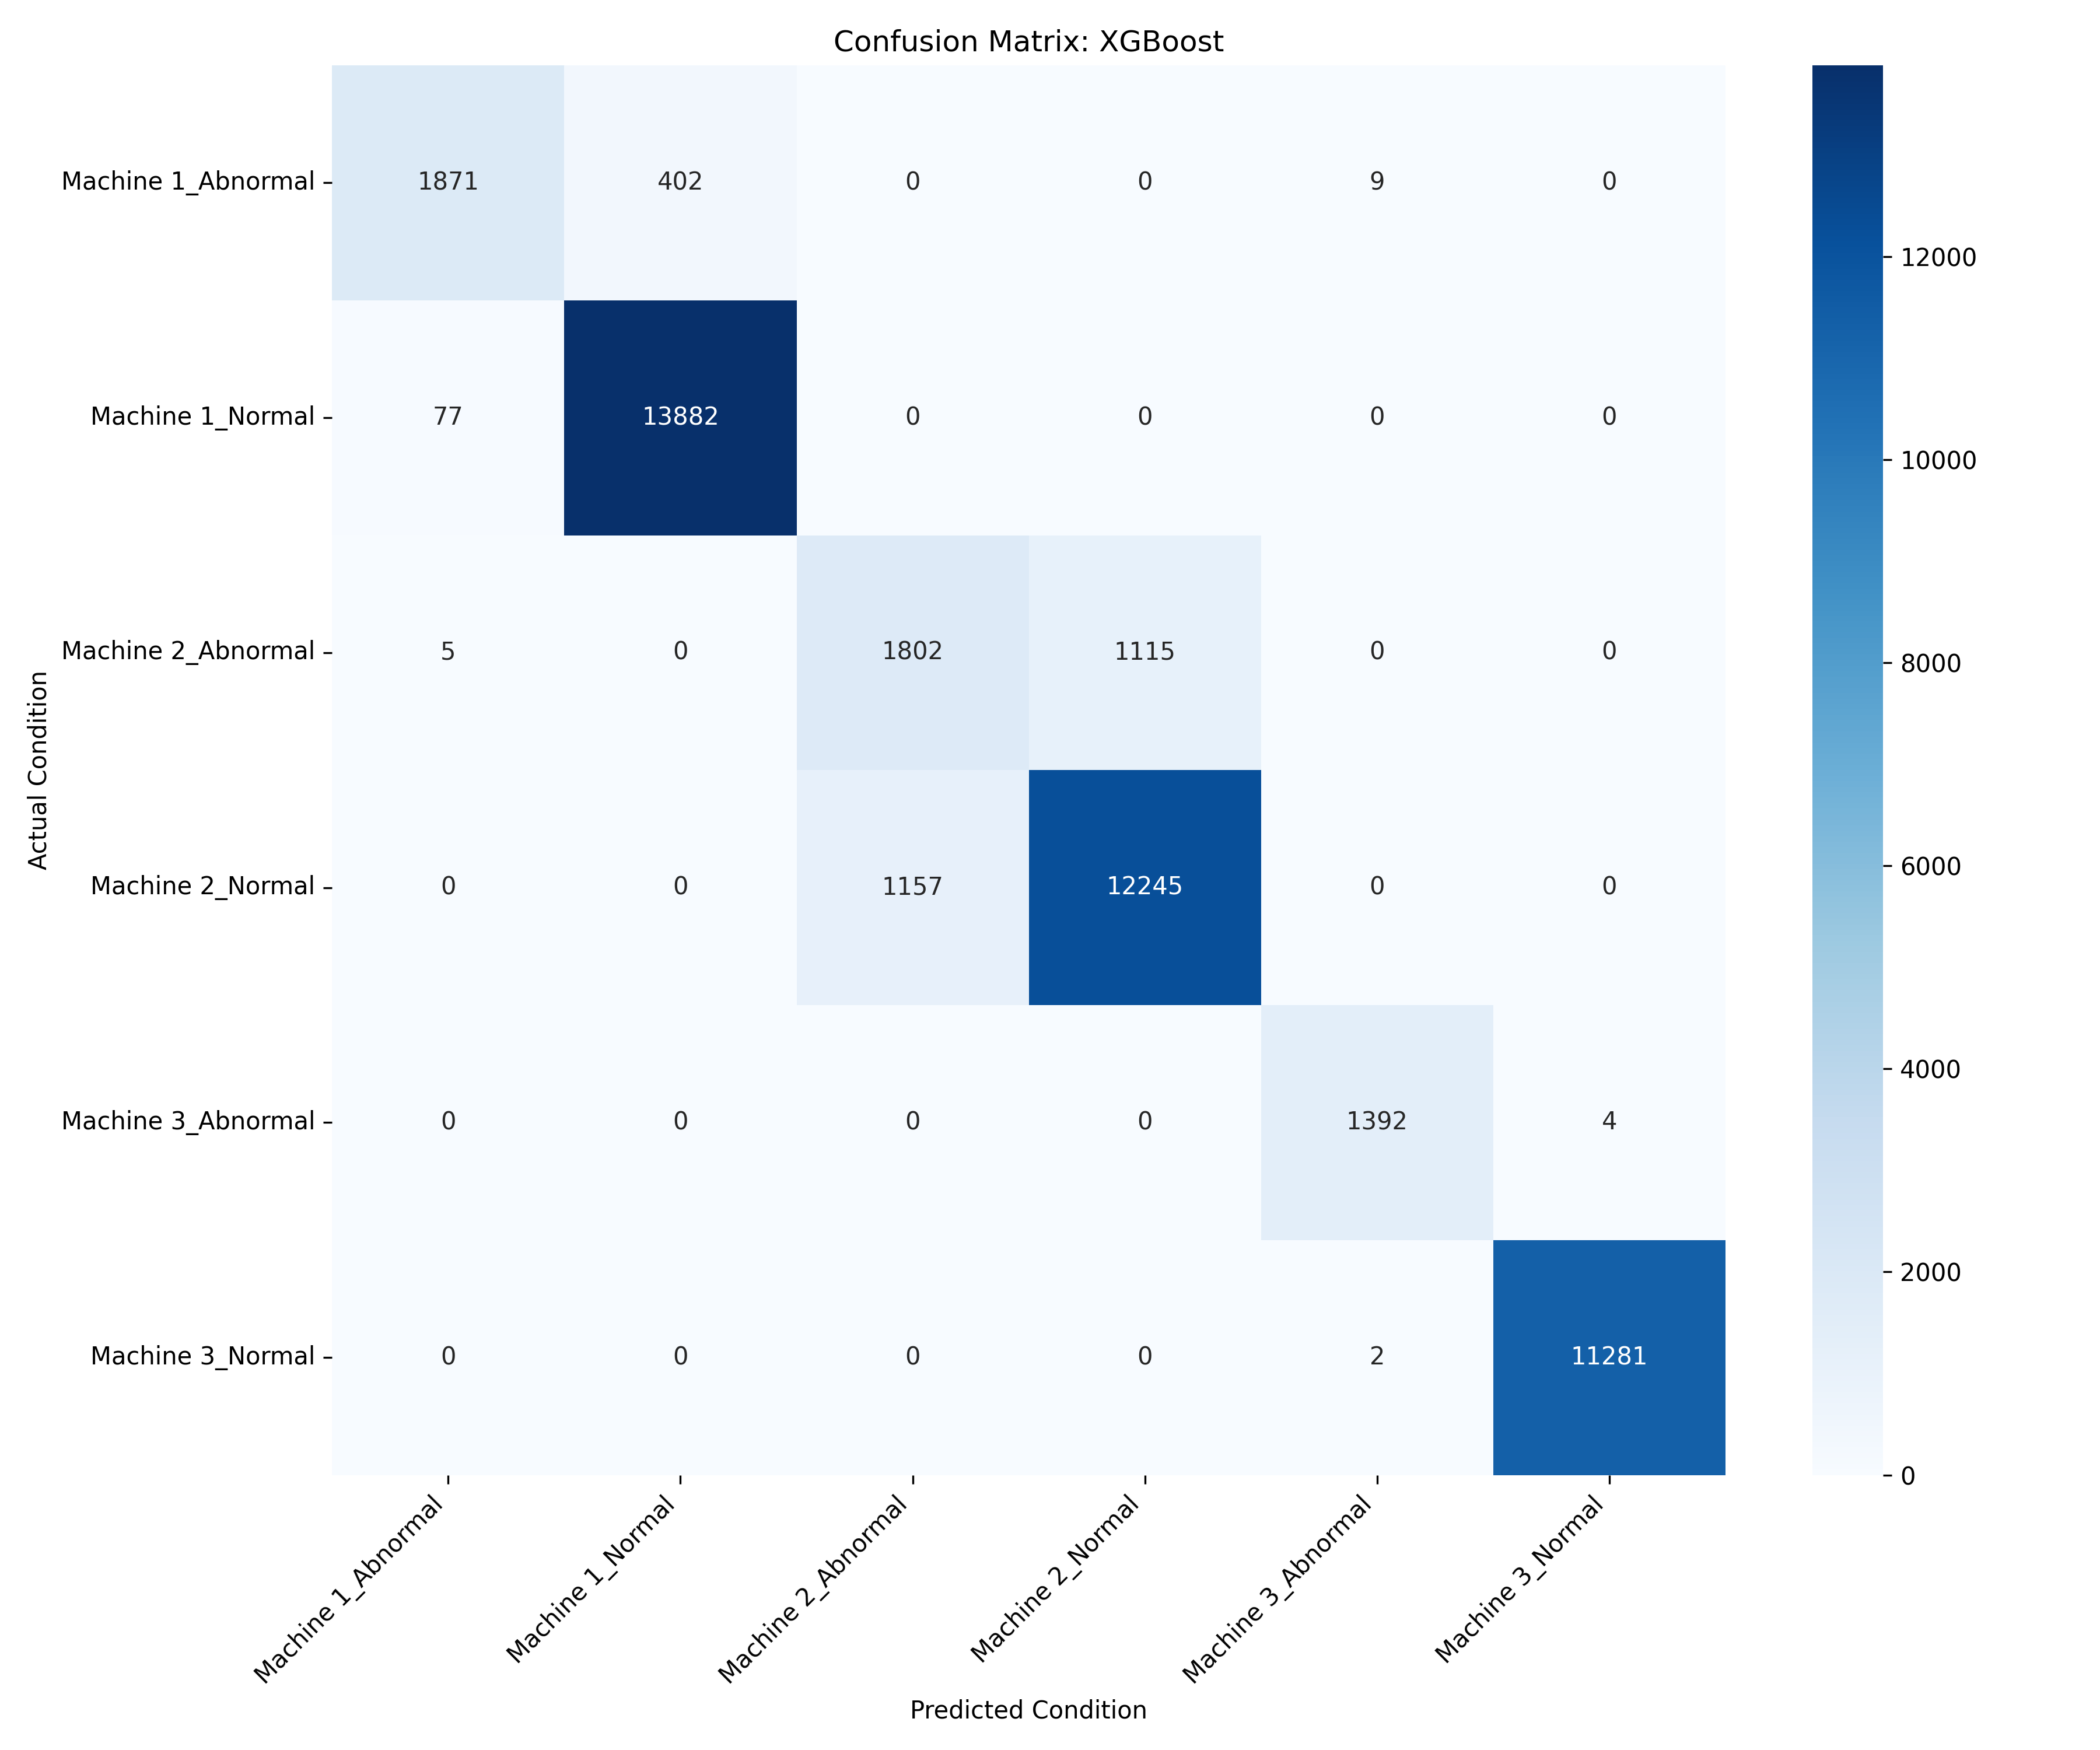
\includegraphics[width=0.8\textwidth]{figures/champion_confusion_matrix.png}
    \caption{Example Diagnostic: Test Set Confusion Matrix}
    \label{fig:conf_matrix}
\end{figure}

These matrices allow engineers to identify specific class-pair confusions (e.g., distinguishing between Machine 1 Normal and Machine 2 Normal) at a glance. Combined with per-class F1-scores, these diagnostics form the basis for our quality assurance gate before any model is promoted to the edge gateways.
